% Competition and evaluation
\section{Competition and evaluation}
\sectionframe{02}{Meet the competition}

\begin{frame}{The task: turn an issue into a working patch}
\tagline{Kaggle gives the agent an issue and a repository before the fix.}
\vspace{4mm}
\begin{tikzpicture}
\path[use as bounding box] (0,-2.05) rectangle (13.35,.38);
\flowlinks
\flowstep{1}{0.0}{Read}{Issue and hints\\Pre-fix repository}
\flowstep{2}{3.5}{Repair}{Edit and test\\Repeat as needed}
\flowstep{3}{7.0}{Export}{Final code changes\\A Git diff patch}
\flowstep{4}{10.5}{Verify}{Clean test run\\PASS / FAIL}
\end{tikzpicture}

\vspace{4mm}
\takeaway{Score = fraction of tasks resolved by the final patches.}
% Sources: \href{https://www.kaggle.com/competitions/gemma-4-developer-agent/overview/evaluation}{Official Evaluation}; docs/overview.md.
\note{Each task is evaluated in a clean environment with the official verification tests. A convincing explanation or a syntactically valid patch is insufficient: the required checks must pass. The agent may iterate within its budget, but only the resulting repair is graded.}
\end{frame}

\begin{frame}{Our entry tells Gemma how to work}
\begin{columns}[c,onlytextwidth]
\column{.48\textwidth}\eyebrow{ONE AGENT ZIP}
\small Instructions and settings tell the agent how to search, edit, and test.\par\vspace{3mm}
An optional learned adapter adds training updates.\par\vspace{3mm}
\textbf{Training is optional.}\par Our scored starting agent uses instructions and settings.
\column{.47\textwidth}

\includegraphics[width=\linewidth]{assets/illustrations/gemma-4.png}\par\vspace{2mm}
\small\textbf{Required model}\par Official quantized Gemma 4 31B.
\end{columns}
\vspace{4mm}
\small\textbf{Upload ZIP} $\longrightarrow$ \textbf{Run agent on each issue} $\longrightarrow$ \textbf{Generate and grade patches}\par\vspace{2mm}
\small Reuse the same agent configuration for every task; put \pathcode{agent.yaml} at the ZIP root.
% Sources: Official Evaluation and Model Selection, Budget and Harness Rules; configs/baseline/.
\note{The base model is fixed to gemma-4-31b-it-qat-w4a16-ct. Quantization compresses model weights for inference. The agent configuration and runtime coordinate calls to that model and tools. Kaggle calls its runner the harness. Optional adapters must obey the model-selection and package rules. Our scored baseline contains no LoRA adapter. The complete accepted file structure is in configs/baseline and the submission guide.}
\end{frame}

\begin{frame}{Public data: 129 tasks across four repositories}
\begin{columns}[T,onlytextwidth]
\column{.49\textwidth}
\begin{tikzpicture}\begin{axis}[xbar,width=6.0cm,height=4.2cm,xmin=0,xmax=75,
 symbolic y coords={HTTPX,Requests,Rich,FastAPI},ytick=data,
 tick label style={font=\small,text=ink},axis x line=bottom,axis y line*=left,
 y axis line style={draw=none},ytick style={draw=none},xtick={0,20,40,60},
 xmajorgrids,grid style={line},bar width=11pt,nodes near coords,point meta=x,
 nodes near coords style={font=\small,anchor=west}]
\addplot[fill=orange,draw=none] coordinates {(1,HTTPX) (13,Requests) (48,Rich) (67,FastAPI)};
\end{axis}\end{tikzpicture}
\column{.47\textwidth}\eyebrow{WHAT IS INCLUDED?}
\begin{itemize}\setlength\itemsep{3mm}\small
\item Issue descriptions and source snapshots
\item Reference fixes and verification tests
\item Search data and runtime packages
\item Example agent and setup guide
\end{itemize}
\end{columns}
\takeaway{Most examples come from FastAPI and Rich. Try other repositories too.}
% Sources: Official Data; resource/manifests/data-audit.json; docs/data.md.
\note{The downloaded package has 524 files totaling 20.88 GiB. It contains 129 task snapshots, but graph and vector files cover 127 unique repository/commit pairs. Reference fixes and test patches are labels for training or controlled evaluation, not inputs to the repair agent. Detailed field definitions, counts, and file mappings are in docs/data.md.}
\end{frame}

\begin{frame}{How do we know an improvement is real?}
\begin{columns}[T,onlytextwidth]
\column{.47\textwidth}\eyebrow[teal]{CHECK THE TEST FIRST}
\small Original code reproduces the bug.\par\vspace{3mm}
The reference repair passes the same check.\par\vspace{4mm}
\textbf{Agent input:} the issue, original code, and tools.
\column{.48\textwidth}\eyebrow{KEEP THE FINAL CHECK FAIR}
\softpanel{orange}{Example split}{
Related code snapshots $\longrightarrow$ training set\par\vspace{2mm}
A different repository $\longrightarrow$ evaluation set}
\small Use held-out answers only for grading.
\end{columns}
\vspace{3mm}
\takeaway{A near-duplicate repair can inflate the score. Fresh tasks test whether the idea transfers.}
% Sources: Official Data; organizer discussions \href{https://www.kaggle.com/competitions/gemma-4-developer-agent/discussion/744951}{744951} and \href{https://www.kaggle.com/competitions/gemma-4-developer-agent/discussion/743817}{743817}. Validation design is our proposal.
\note{Validation is the task set used to compare choices before final submission. Do not let the model read reference patches or verification answers at inference. A failing environment can make a correct repair look wrong; empty and gold controls help detect this. Group related snapshots rather than randomly scattering near-duplicates across train and validation. Cross-repository evaluation measures a stronger form of generalization; hidden tasks use private repositories.}
\end{frame}

\begin{frame}{The competition gives us four L4 GPUs}
\begin{columns}[c,onlytextwidth]
\column{.40\textwidth}
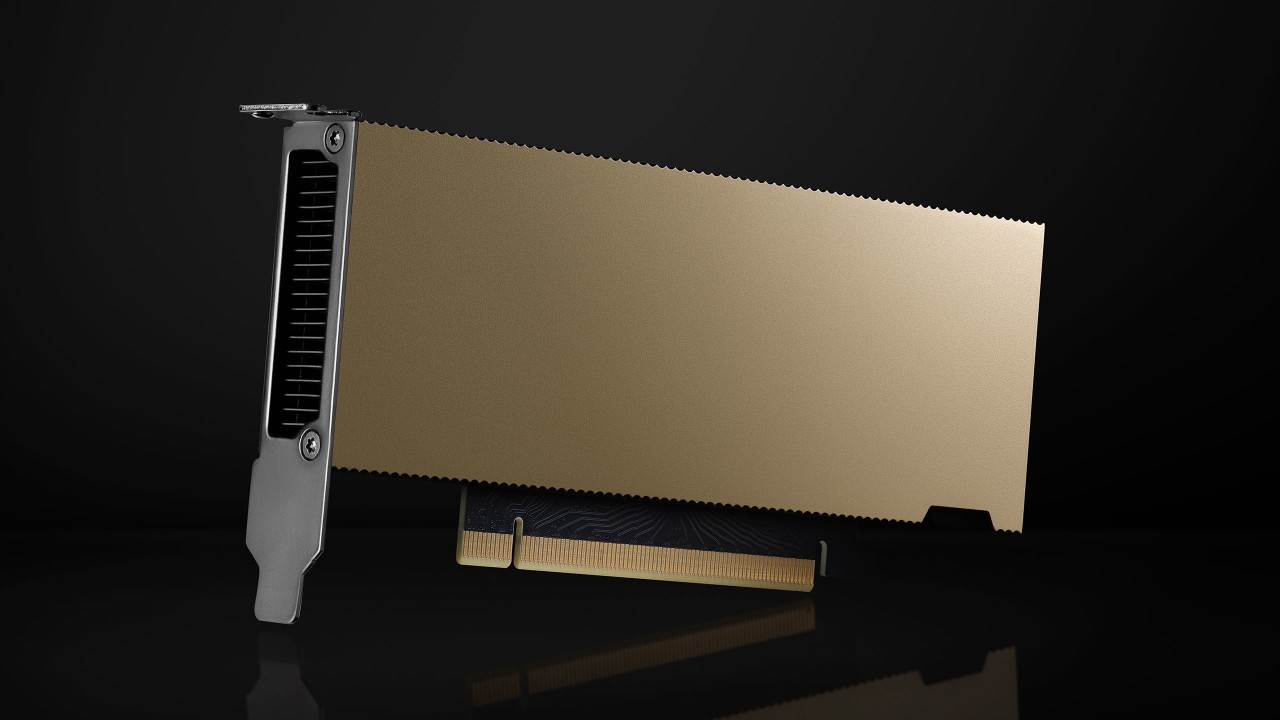
\includegraphics[width=\linewidth]{assets/illustrations/nvidia-l4.jpg}\par\vspace{2mm}
{\color{orange}\LARGE\bfseries 4 $\times$ L4}\quad\small 24 GB each
\column{.55\textwidth}
\small\renewcommand{\arraystretch}{1.45}
\begin{tabularx}{\linewidth}{@{}lX@{}}
\textbf{32,768 tokens} & Text per model call\\
\textbf{12 hours} & Setup and patch generation\\
\textbf{Under 3 GiB} & Unpacked submission size
\end{tabularx}
\end{columns}
\vspace{4mm}
\small Tokens are pieces of text. The context holds the issue, conversation, tool results, and response.\par
\vspace{2mm}
\takeaway{About 120 hidden tasks means roughly six minutes per repair, before overhead.}
% Sources: Official Upgraded Accelerators, Evaluation, and model/budget rules; discussions 744258 and 743063. The 12-hour limit excludes verification.
\note{VRAM is memory on the GPU, used for model weights and inference state. Total memory across four GPUs is not automatically a single contiguous allocation. The official runtime handles model distribution. The context limit is per request, not a lifetime total for the task. Twelve hours covers setup and sequential patch generation, excluding final verification; six minutes is only an average from organizer estimates, not a guaranteed per-task allowance. Our tested agent has its own stricter per-task budget.}
\end{frame}

\begin{frame}{Your first Kaggle session}
\begin{columns}[T,onlytextwidth]
\column{.57\textwidth}
\eyebrow{OPEN THE OFFICIAL STARTER}
\begin{enumerate}\setlength\itemsep{3mm}\small
\item Copy the \href{https://www.kaggle.com/code/ryanholbrook/getting-started-gemma-4-developer-agent}{Getting Started notebook}.
\item Attach data, packages, and the required model.
\item Select \textbf{L4 $\times$ 4} and \textbf{Internet off}.
\item Try a few tasks; read the patches and tests.
\end{enumerate}
\column{.38\textwidth}
\softpanel{orange}{Check GPU time first}{
Check your remaining GPU quota before starting. L4 $\times$ 4 uses twice the T4 $\times$ 2 / P100 reference rate.}
\vspace{1mm}
\small The scored run has its own 12-hour budget.
\end{columns}
% Sources: Official starter and Upgraded Accelerators; source text checked through the Kaggle API on October 5, 2026.
\note{A notebook is an interactive document containing executable cells. The official wheelhouse supplies Python packages for evaluation. The old quota reference is T4 x2 or P100. Check the account quota before another run; its available balance changes. Offline execution means inputs must already be attached. We have already completed a private L4 notebook; this page is a reproducible entry point for teammates, not a claim that another run is still queued.}
\end{frame}


\begin{frame}{A first exercise: follow one repair from start to finish}
\tagline{In the official starter, complete setup and start the model server first.}
\begin{columns}[T,onlytextwidth]
\column{.51\textwidth}\eyebrow[teal]{CHOOSE ONE TASK IN SECTION 5}
\small Replace the \pathcode{SAMPLE_TASKS} selection:\par\vspace{2mm}
\softpanel{teal}{One public example}{
\pathcode{SAMPLE_TASKS = [t for t in tasks}\par
\pathcode{if t.instance_id == "rich_3454"]}}
\column{.44\textwidth}\eyebrow{RUN AND INSPECT}
\small Run the inference and verification cell.\par\vspace{2mm}
Read the tool log, final patch, and test result.\par\vspace{2mm}
Change one instruction; repeat the same task to learn the workflow.
\end{columns}
\vspace{3mm}
\takeaway{Finish with a patch and verification result.\\Use shared held-out tasks for later comparisons.}
% Sources: archived official starter, Section 5, SAMPLE_TASKS and evaluator loop. Exercise is a suggested onboarding workflow.
\note{The archived starter uses tasks[:2] as its default sample. The displayed Python list comprehension selects exactly rich_3454 from the loaded tasks and can span two lines inside brackets. Run setup, model serving, and compiler preparation before the evaluation cell. Setup package versions may need the fixes documented in docs/training-plan.md and our validated runtime notebook; this slide does not assert that an unmodified upstream starter reproduces our score. A completed exercise has a generated patch and an interpretable verification result, whether pass or fail. Inspect a failure before modifying prompts. Repeating a known task teaches the workflow; use separate evaluation tasks for research claims. GPU time continues while the session is active: save useful outputs and stop it when done.}
\end{frame}

\begin{frame}{Leaderboard snapshot: best 24\%, median 8\%}
\tagline{October 5, 2026, 03:50 UTC / 1,755 scored teams / public leaderboard}
\begin{columns}[T,onlytextwidth]
\column{.65\textwidth}
\begin{tikzpicture}\begin{axis}[ybar,width=8.7cm,height=4.5cm,ymin=0,ymax=390,
 symbolic x coords={0,1,3,5,6,8,10,12,13,15,17,24},xtick=data,
 tick label style={font=\scriptsize},axis x line=bottom,axis y line=left,
 ymajorgrids,grid style={line},bar width=10pt,
 xlabel={Displayed resolution rate (\%)},ylabel={Teams},label style={font=\small}]
\addplot[fill=teal,draw=none] coordinates {(0,133) (1,55) (3,65) (5,148) (6,200) (8,316) (10,344) (12,307) (13,139) (15,41) (17,6) (24,1)};
\end{axis}\end{tikzpicture}
\column{.31\textwidth}\eyebrow{HOW TO READ IT}
\small Many teams are tied. A few solved tasks can move the rank.\par
\vspace{3mm}\alert{Use local tests to understand why an idea helps.}
\end{columns}
% Sources: Official leaderboard CSV; resource/leaderboard/summary.json. Discrete score categories preserve the CSV's displayed precision.
\end{frame}

\begin{frame}{Our first milestone: a scored agent and a repair}
\begin{columns}[T,onlytextwidth]
\column{.43\textwidth}\eyebrow{OFFICIAL PUBLIC SCORE}
{\color{orange}\fontsize{38}{42}\selectfont\bfseries 0.12}\par\vspace{3mm}
\small Our baseline submission completed successfully.\par\vspace{2mm}
\textbf{12\%} public resolution rate.
\column{.51\textwidth}\eyebrow[teal]{A COMPLETED KAGGLE REPAIR}
\small Run on \textbf{4 NVIDIA L4 GPUs}.\par\vspace{2mm}
Public task \texttt{rich\_3454}:\par\vspace{1mm}
{\color{orange}\Large\bfseries 84 tests passed}\par\vspace{3mm}
Agent phase: \textbf{74.10 seconds}.\par
{\footnotesize\color{muted}One task; timing excludes model startup.}
\end{columns}
\vspace{6mm}
\takeaway{Next: evaluate more tasks and try our first small training experiment.}
% Sources: Authenticated Kaggle API, October 5, 2026, 18:30 UTC; downloaded L4 hardware, controls, inference and test logs. See resource/manifests/competition-result.json and kaggle-runtime-smoke.json.
\note{Both existing remote tasks were rechecked at 18:30 UTC on October 5, 2026; both are COMPLETE with no error. The official submission public score is 0.12, or 12 percent; no private score is returned. The separate L4 notebook ran one real public task. Its unmodified-code control had one failure and 82 passes; the reference fix passed 83 tests; the agent patch passed 84. The agent phase took 74.101 seconds and excluded model startup. These are different measurements: 84 passing tests is not 84 solved competition tasks. The L4-produced ZIP matches the uploaded baseline archive. There is no full local benchmark or validated training run yet.}
\end{frame}

\begin{frame}{A reading map for the team}
\eyebrow[teal]{START WITH THREE THINGS}
\small Competition rules\quad$\longrightarrow$\quad Official starter\quad$\longrightarrow$\quad Our first result
\vspace{6mm}
\begin{columns}[T,onlytextwidth]
\column{.30\textwidth}\softpanel{orange}{112 notebooks}{Find ideas and code examples.}
\column{.30\textwidth}\softpanel{teal}{116 discussions}{Read organizer answers and lessons.}
\column{.30\textwidth}\softpanel{orange}{4 model cards}{Understand available model resources.}
\end{columns}
\vspace{3mm}
\small Open \pathcode{resource/README.md} for the October 5 archive and review notes.
% Sources: Project resource/ indexes for official pages, notebooks, discussions, and models; October 5, 2026 snapshot.
\note{This is a dated snapshot, not a claim that the live website will always have these counts. The Code review has 112 records; one returned an empty source and cannot be inspected. The discussion archive contains 370 posts/replies across 116 topics. Model cards on a competition page do not override the required base-model rule. Public notebook scores are authors	extquotesingle{} claims until independently reproduced.}
\end{frame}
